\documentclass[11pt,a4paper]{article}

\usepackage[margin=0.85in]{geometry}
\usepackage[T1]{fontenc}
\usepackage[utf8]{inputenc}
\usepackage{lmodern}
\usepackage{microtype}
\usepackage{amsmath,amssymb}
\usepackage{booktabs}
\usepackage{array}
\usepackage{hyperref}
\usepackage{xcolor}
\usepackage{tikz}
\usepackage{pgfplots}
\pgfplotsset{compat=1.18}
\usetikzlibrary{arrows.meta,positioning,shapes.geometric,fit}

\definecolor{navy}{HTML}{1B365D}
\definecolor{teal}{HTML}{008080}
\definecolor{amber}{HTML}{D97706}
\definecolor{crimson}{HTML}{B91C1C}
\definecolor{slate}{HTML}{475569}

\hypersetup{
  colorlinks=true,
  linkcolor=navy,
  urlcolor=teal,
  pdftitle={Fault-Tolerant, Experiment-Preserving Multi-GPU Diffusion Inference over Tailscale},
  pdfauthor={Muadib Networking Study}
}

\title{\textbf{Fault-Tolerant, Experiment-Preserving Multi-GPU Diffusion Inference over Tailscale and SSH}}
\author{Muadib Distributed Inference \& Networking Report}
\date{25 November 2026}

\begin{document}
\maketitle

\begin{abstract}
We describe a checkpoint-aware, resumable diffusion-inference system that sends independent image jobs from a CPU coordinator to heterogeneous laptops over SSH and Tailscale. A frozen plan retains job and stratum identities, while an attempt journal and uncertain-work quarantine retain incomplete work across failures. A five-peer echo pilot measured application RTT and RTT variation on coordinator-to-peer paths. In single, non-interleaved runs on a 36-job plan, the recorded dispatch segment was $51.73\,\text{s}$ on \texttt{gpu-3} alone and $46.50\,\text{s}$ with three workers, a descriptive ratio of $1.11\times$. This observation is not evidence of a general speedup. The recovery ledger records one uncertain EOF, followed by a resume that reused 35 verified images and completed the remaining job. A separately retained Linux eBPF recheck reported zero port-22 retransmission events over a requested three-second interval; event loss and exact attachment times were not measured.
\end{abstract}

\section{Overview and Motivation}
Evaluating diffusion models across controlled experimental conditions (e.g., color, seed, and stratum quotas) requires generating balanced image sets without silently dropping hard seeds or mixing incompatible checkpoints. In an academic lab or student setting, compute is often fragmented across personal laptops on different operating systems (Windows and Linux) connected over campus Wi-Fi and a Tailscale overlay network.

This project builds a lightweight Python coordinator--worker system (\texttt{ops/}) that turns heterogeneous laptops into a reliable, resumable inference cluster over authenticated SSH tunnels, without requiring Kubernetes, shared filesystems, or root privileges on remote workers.

\begin{figure}[ht]
\centering
\resizebox{0.98\textwidth}{!}{%
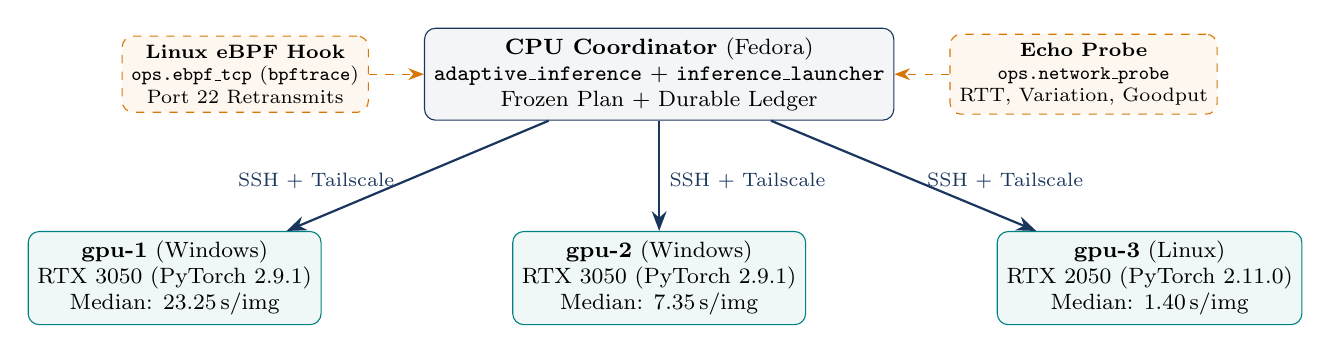
\begin{tikzpicture}[
  node distance=1.0cm and 0.5cm,
  box/.style={draw=navy, rounded corners=4pt, fill=navy!5, minimum width=2.9cm, minimum height=0.95cm, align=center, font=\footnotesize},
  worker/.style={draw=teal, rounded corners=4pt, fill=teal!6, minimum width=3.1cm, minimum height=1.05cm, align=center, font=\footnotesize},
  probe/.style={draw=amber, dashed, rounded corners=4pt, fill=amber!6, minimum width=2.4cm, minimum height=0.8cm, align=center, font=\scriptsize},
  arr/.style={-{Stealth[length=2.5mm]}, thick, navy},
  darr/.style={-{Stealth[length=2mm]}, dashed, amber}
]
  \node[box] (coord) {\textbf{CPU Coordinator} (Fedora)\\\texttt{adaptive\_inference} + \texttt{inference\_launcher}\\Frozen Plan + Durable Ledger};
  \node[probe, left=0.7cm of coord] (ebpf) {\textbf{Linux eBPF Hook}\\\texttt{ops.ebpf\_tcp} (\texttt{bpftrace})\\Port 22 Retransmits};
  \node[probe, right=0.7cm of coord] (echo) {\textbf{Echo Probe}\\\texttt{ops.network\_probe}\\RTT, Variation, Goodput};

  \node[worker, below left=1.4cm and 1.3cm of coord] (g1) {\textbf{gpu-1} (Windows)\\RTX 3050 (PyTorch 2.9.1)\\Median: $23.25\,\text{s/img}$};
  \node[worker, below=1.4cm of coord] (g2) {\textbf{gpu-2} (Windows)\\RTX 3050 (PyTorch 2.9.1)\\Median: $7.35\,\text{s/img}$};
  \node[worker, below right=1.4cm and 1.3cm of coord] (g3) {\textbf{gpu-3} (Linux)\\RTX 2050 (PyTorch 2.11.0)\\Median: $1.40\,\text{s/img}$};

  \draw[arr] (coord) -- node[left, font=\scriptsize, pos=0.55] {SSH + Tailscale} (g1);
  \draw[arr] (coord) -- node[right, font=\scriptsize, pos=0.55] {SSH + Tailscale} (g2);
  \draw[arr] (coord) -- node[right, font=\scriptsize, pos=0.55] {SSH + Tailscale} (g3);
  \draw[darr] (ebpf) -- (coord);
  \draw[darr] (echo) -- (coord);
\end{tikzpicture}%
}
\caption{System architecture: a CPU-only coordinator dispatches frozen-plan diffusion jobs over authenticated SSH local-forwarding tunnels across Tailscale to heterogeneous Windows and Linux GPU workers, complemented by echo probing and Linux eBPF telemetry.}
\label{fig:arch}
\end{figure}

\section{Novelty and Systems Contributions}
While adaptive edge scheduling and distributed diffusion have prior art (e.g., RISE, EAT, DistriFusion), our system targets a distinct intersection of \textbf{networking reliability} and \textbf{scientific experimental validity}:
\begin{enumerate}
  \item \textbf{Experiment-Preserving Frozen Plans:} Rather than treating jobs as fungible or dropping stragglers, \texttt{ops.adaptive\_inference} freezes the logical job set (\texttt{id}, \texttt{stratum}, \texttt{checkpoint\_\allowbreak sha256}, \texttt{color}, \texttt{seed}) before execution. Scheduling may reorder or reassign jobs across workers, but never alters sample composition or stratum quotas.
  \item \textbf{Uncertain-Work Quarantine:} A client timeout or broken SSH tunnel does not stop a remote GPU job. Instead of silently launching a duplicate job, the coordinator marks the attempt \emph{uncertain}, quarantines the worker for the remainder of the session, archives any torn final journal line byte-for-byte, and requires explicit \texttt{--allow-uncertain-\allowbreak retry} during \texttt{--resume}. Local PNG/disk publication failures are separated from uncertain remote failures.
  \item \textbf{PID-Free SSH-Owned Worker Lifecycle (\texttt{ops.remote\_worker}):} Remote workers verify the checkpoint SHA-256 before binding loopback, emit a random per-launch ownership token, and self-terminate on SSH \texttt{stdin} EOF or a bounded lease timer---never killing processes by PID or port. On Windows, a non-blocking \texttt{PeekNamedPipe} watchdog avoids a reproducible Windows NumPy native-import deadlock caused by blocking \texttt{stdin} reads in a background thread.
  \item \textbf{Independent Artifact Verification \& Multi-Layer Observability:} Every completed job is verified by PNG structure, dimensions, and SHA-256 digest (\texttt{ops.benchmark\_report} with \texttt{--verify-results}). The instrumentation can observe network behavior at three layers: coordinator request round-trip duration, SSH-forwarded TCP echo RTT/RTT variation/goodput (\texttt{ops.network\_probe}), and host-level Linux \texttt{tcp\_retransmit\_skb} tracepoint via \texttt{bpftrace} (\texttt{ops.ebpf\_tcp}).
\end{enumerate}

\section{Experimental Setup and Network Telemetry}
\subsection{Hardware and Software Environment}
The inference experiments used the same 480,000-update PilotUNet EMA warmstart checkpoint (SHA-256 prefix \texttt{f29d75e9...cf459}). The coordinator ran on a CPU-only Fedora Linux laptop; three remote GPU laptops participated over Tailscale:
\begin{itemize}
  \item \textbf{gpu-1} (Windows, RTX~3050, PyTorch 2.9.1+cu128)
  \item \textbf{gpu-2} (Windows, RTX~3050, PyTorch 2.9.1+cu128)
  \item \textbf{gpu-3} (NewAurora, Linux, RTX~2050, PyTorch 2.11.0+cu128)
\end{itemize}
Two additional Tailscale peers were included in the network probe, while GPU inference used the three verified workers.

\subsection{Five-Host Echo Probe Measurements}
Each peer was probed with 20 sequential 1,024-byte TCP echo requests ($150\,\text{ms}$ gap, $3\,\text{s}$ per-operation socket timeout in the then-current probe) through an SSH local-forwarding tunnel over Tailscale. All 100/100 probes succeeded ($0\%$ failure). Figure~\ref{fig:echo} and Table~\ref{tab:echo} summarize RTT, p95, RTT variation (successive absolute differences), and echoed-payload goodput. These legacy probes used zero-filled payloads; the server-side timeout is not recorded. Peer windows were staggered by several minutes. Goodput includes pacing and is not link capacity.

\begin{figure}[ht]
\centering
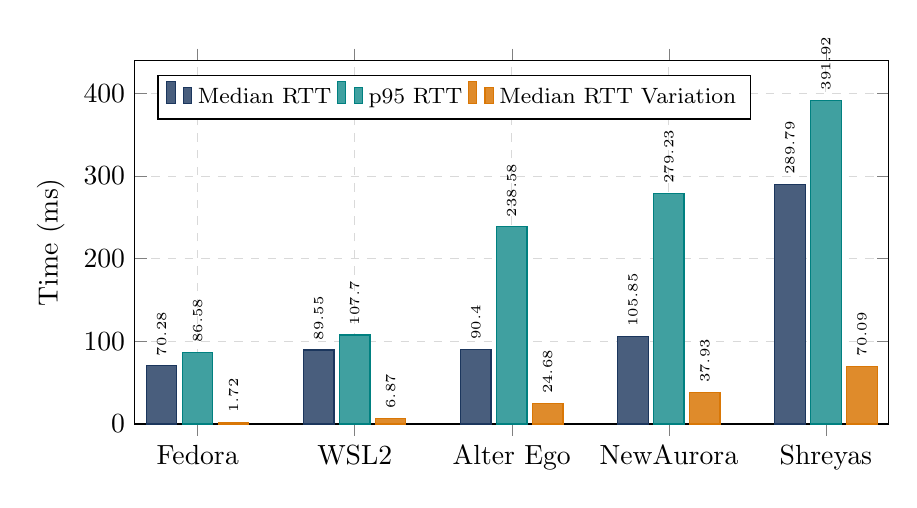
\begin{tikzpicture}
\begin{axis}[
  ybar,
  bar width=11pt,
  width=0.92\textwidth,
  height=6.2cm,
  ylabel={Time (ms)},
  symbolic x coords={Fedora, WSL2, Alter Ego, NewAurora, Shreyas},
  xtick=data,
  ymin=0,
  ymax=440,
  legend style={at={(0.03,0.96)}, anchor=north west, legend columns=3, font=\footnotesize},
  grid=major,
  grid style={dashed, gray!30},
  nodes near coords,
  every node near coord/.append style={font=\tiny, rotate=90, anchor=west}
]
  \addplot[fill=navy!80, draw=navy] coordinates {(Fedora,70.28) (WSL2,89.55) (Alter Ego,90.40) (NewAurora,105.85) (Shreyas,289.79)};
  \addplot[fill=teal!75, draw=teal] coordinates {(Fedora,86.58) (WSL2,107.70) (Alter Ego,238.58) (NewAurora,279.23) (Shreyas,391.92)};
  \addplot[fill=amber!85, draw=amber] coordinates {(Fedora,1.72) (WSL2,6.87) (Alter Ego,24.68) (NewAurora,37.93) (Shreyas,70.09)};
  \legend{Median RTT, p95 RTT, Median RTT Variation}
\end{axis}
\end{tikzpicture}
\caption{Five-host Tailscale SSH echo probe latencies ($n=20$ per host, $1{,}024\,\text{B}$ payload, $100\%$ success).}
\label{fig:echo}
\end{figure}

\begin{table}[ht]
\centering
\small
\resizebox{\textwidth}{!}{%
\begin{tabular}{lrrrrr}
\toprule
\textbf{Endpoint} & \textbf{Success} & \textbf{Median RTT (ms)} & \textbf{p95 RTT (ms)} & \textbf{Median Var.\ (ms)} & \textbf{Goodput (Mbps)} \\
\midrule
Fedora (Linux) & 20/20 & 70.28 & 86.58 & 1.72 & 0.0381 \\
Nikhil (WSL2) & 20/20 & 89.55 & 107.70 & 6.87 & 0.0351 \\
Alter Ego (\texttt{gpu-1}) & 20/20 & 90.40 & 238.58 & 24.68 & 0.0315 \\
NewAurora (\texttt{gpu-3}) & 20/20 & 105.85 & 279.23 & 37.93 & 0.0283 \\
Shreyas (\texttt{gpu-2}) & 20/20 & 289.79 & 391.92 & 70.09 & 0.0184 \\
\bottomrule
\end{tabular}%
}
\caption{Application-level TCP echo telemetry over SSH/Tailscale (paced $150\,\text{ms}$ interval; includes SSH and endpoint processing).}
\label{tab:echo}
\end{table}

\section{Multi-GPU Inference Performance Results}
We evaluated frozen balanced plans (\texttt{low-balanced} stratum, alternating \texttt{red} and \texttt{blue} seeds) across 18-job and 36-job workloads, comparing \texttt{gpu-3} alone against 3-GPU \texttt{round-robin} and 3-GPU \texttt{adaptive} scheduling. All runs achieved $100\%$ completion ($0$ missing) and passed PNG and SHA-256 verification. Dispatch timings exclude worker startup, teardown and setup. The first recorded \texttt{gpu-3} request in each 36-job run was about $2.3\,\text{s}$ versus roughly $1.4\,\text{s}$ for subsequent requests; the cause was not measured.

\begin{figure}[ht]
\centering
\begin{minipage}[t]{0.48\textwidth}
\centering
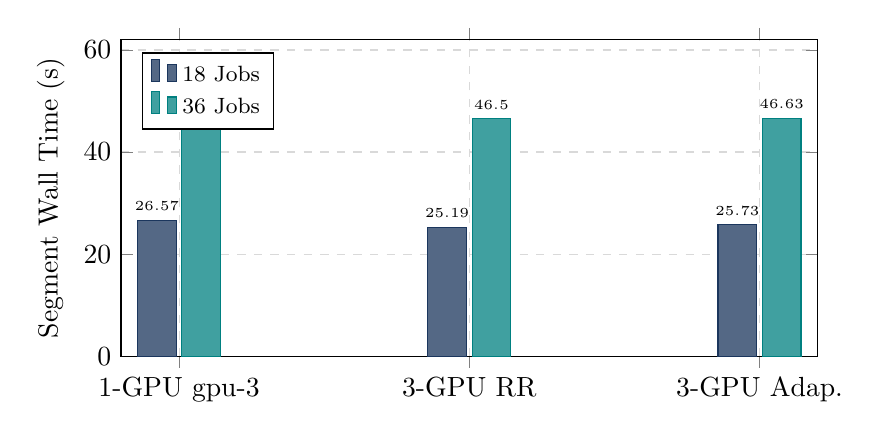
\begin{tikzpicture}
\begin{axis}[
  ybar,
  bar width=14pt,
  width=0.86\textwidth,
  height=5.6cm,
  ylabel={Segment Wall Time (s)},
  symbolic x coords={1-GPU gpu-3, 3-GPU RR, 3-GPU Adap.},
  xtick=data,
  ymin=0,
  ymax=62,
  legend style={at={(0.03,0.96)}, anchor=north west, font=\footnotesize},
  grid=major,
  grid style={dashed, gray!30},
  nodes near coords,
  every node near coord/.append style={font=\tiny}
]
  \addplot[fill=navy!75, draw=navy] coordinates {(1-GPU gpu-3,26.57) (3-GPU RR,25.19) (3-GPU Adap.,25.73)};
  \addplot[fill=teal!75, draw=teal] coordinates {(1-GPU gpu-3,51.73) (3-GPU RR,46.50) (3-GPU Adap.,46.63)};
  \legend{18 Jobs, 36 Jobs}
\end{axis}
\end{tikzpicture}
\end{minipage}\hfill
\begin{minipage}[t]{0.48\textwidth}
\centering
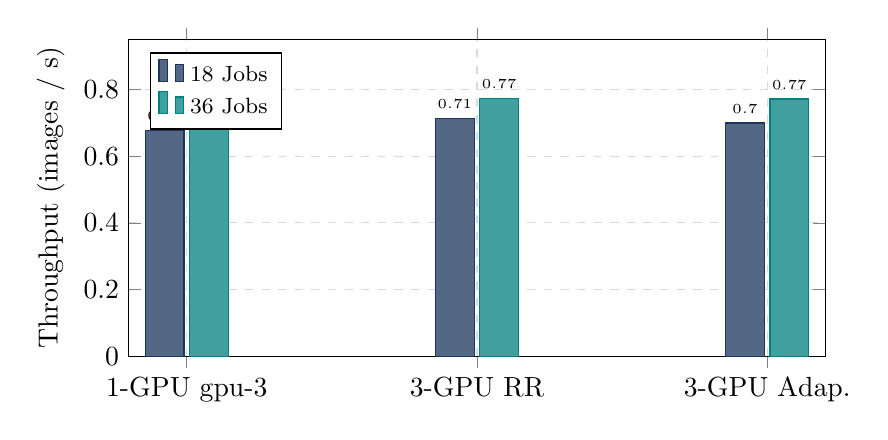
\begin{tikzpicture}
\begin{axis}[
  ybar,
  bar width=14pt,
  width=0.86\textwidth,
  height=5.6cm,
  ylabel={Throughput (images / s)},
  symbolic x coords={1-GPU gpu-3, 3-GPU RR, 3-GPU Adap.},
  xtick=data,
  ymin=0,
  ymax=0.95,
  legend style={at={(0.03,0.96)}, anchor=north west, font=\footnotesize},
  grid=major,
  grid style={dashed, gray!30},
  nodes near coords,
  every node near coord/.append style={font=\tiny}
]
  \addplot[fill=navy!75, draw=navy] coordinates {(1-GPU gpu-3,0.677) (3-GPU RR,0.714) (3-GPU Adap.,0.700)};
  \addplot[fill=teal!75, draw=teal] coordinates {(1-GPU gpu-3,0.696) (3-GPU RR,0.774) (3-GPU Adap.,0.772)};
  \legend{18 Jobs, 36 Jobs}
\end{axis}
\end{tikzpicture}
\end{minipage}
\caption{Makespan (left, lower is better) and throughput (right, higher is better) for 18-job and 36-job frozen plans. The observed 36-job ratio relative to \texttt{gpu-3} alone is $1.11\times$; each configuration was run once.}
\label{fig:makespan}
\end{figure}

\begin{table}[ht]
\centering
\small
\begin{tabular}{llrrrrrr}
\toprule
\textbf{Run} & \textbf{Policy / Nodes} & \textbf{Comp.} & \textbf{Wall (s)} & \textbf{Ratio} & \textbf{Img/s} & \textbf{Med.\ (s)} & \textbf{p95 (s)} \\
\midrule
18-job baseline & \texttt{gpu-3} only & 18/18 & 26.573 & $1.00\times$ & 0.677 & 1.418 & 1.574 \\
18-job 3-GPU & \texttt{round-robin} & 18/18 & 25.193 & $1.05\times$ & 0.714 & 1.361 & 11.822 \\
18-job 3-GPU & \texttt{adaptive} & 18/18 & 25.728 & $1.03\times$ & 0.700 & 1.436 & 11.794 \\
\midrule
36-job baseline & \texttt{gpu-3} only & 36/36 & 51.727 & $1.00\times$ & 0.696 & 1.401 & 1.465 \\
36-job 3-GPU & \texttt{round-robin} & 36/36 & 46.504 & $1.11\times$ & 0.774 & 1.405 & 12.484 \\
36-job 3-GPU & \texttt{adaptive} & 36/36 & 46.629 & $1.11\times$ & 0.772 & 1.448 & 12.263 \\
\bottomrule
\end{tabular}
\caption{Recorded dispatch time, its single-run ratio to \texttt{gpu-3} alone, throughput, and request duration quantiles; result files and hashes were verified.}
\label{tab:perf}
\end{table}

\subsection{Heterogeneity, Stragglers, and Policy Behavior}
Figure~\ref{fig:perworker} shows the stark hardware/runtime heterogeneity across the three GPU workers during the 36-job runs: \texttt{gpu-3} completes requests in $1.40\,\text{s}$ median ($28$ jobs), \texttt{gpu-2} in $7.35\,\text{s}$ ($6$ jobs), and \texttt{gpu-1} in $23.25\,\text{s}$ ($2$ jobs). Because both \texttt{round-robin} and \texttt{adaptive} dispatch one in-flight job to whichever worker is idle, \texttt{gpu-3} automatically absorbs $77.8\%$ of the workload under both policies, yielding the exact same $2/6/28$ split. Meanwhile, the slow tail of \texttt{gpu-1} and \texttt{gpu-2} elevates the aggregate p95 request latency from $1.47\,\text{s}$ (\texttt{gpu-3} only) to $12.48\,\text{s}$ (3-GPU), while the observed dispatch segment is $10.1\%$ shorter in this one comparison. The runtimes differ and the comparison was not repeated or interleaved. In the 36-job plans, eight PNG hashes differed between the \texttt{gpu-3}-only and round-robin runs, and twelve differed between the two three-worker policies; every differing job in these comparisons was assigned to a different worker. Equal seeds and checkpoints therefore do not establish bitwise equivalence across these environments.

\begin{figure}[ht]
\centering
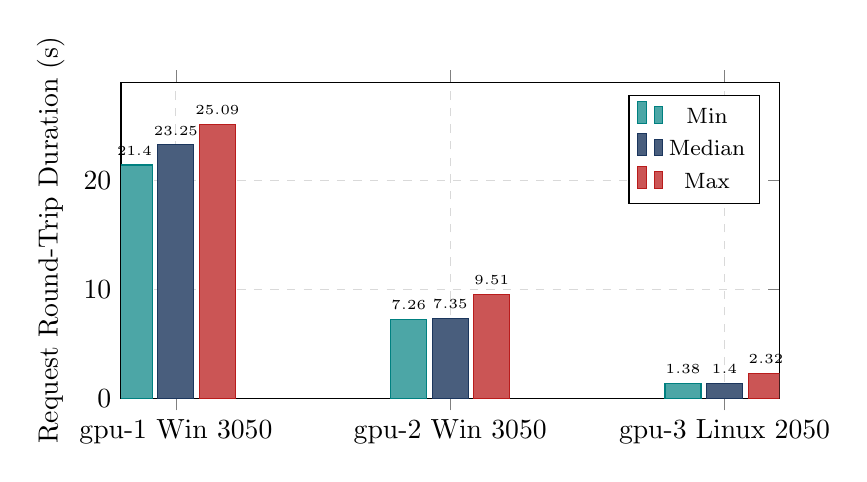
\begin{tikzpicture}
\begin{axis}[
  ybar,
  bar width=13pt,
  width=0.82\textwidth,
  height=5.6cm,
  ylabel={Request Round-Trip Duration (s)},
  symbolic x coords={gpu-1 Win 3050, gpu-2 Win 3050, gpu-3 Linux 2050},
  xtick=data,
  ymin=0,
  ymax=29,
  legend style={at={(0.97,0.96)}, anchor=north east, font=\footnotesize},
  grid=major,
  grid style={dashed, gray!30},
  nodes near coords,
  every node near coord/.append style={font=\tiny}
]
  \addplot[fill=teal!70, draw=teal] coordinates {(gpu-1 Win 3050,21.40) (gpu-2 Win 3050,7.26) (gpu-3 Linux 2050,1.38)};
  \addplot[fill=navy!80, draw=navy] coordinates {(gpu-1 Win 3050,23.25) (gpu-2 Win 3050,7.35) (gpu-3 Linux 2050,1.40)};
  \addplot[fill=crimson!75, draw=crimson] coordinates {(gpu-1 Win 3050,25.09) (gpu-2 Win 3050,9.51) (gpu-3 Linux 2050,2.32)};
  \legend{Min, Median, Max}
\end{axis}
\end{tikzpicture}
\caption{Per-worker request duration spread in the 36-job \texttt{round-robin} run (\texttt{gpu-1}: $n=2$, \texttt{gpu-2}: $n=6$, \texttt{gpu-3}: $n=28$).}
\label{fig:perworker}
\end{figure}

\section{Fault Recovery and eBPF Instrumentation}
\subsection{Controlled Mid-Run Disconnect and Resume}
In the 36-job \texttt{adaptive} run (\texttt{three-gpu-fault-resume-20261125}), the ledger records an EOF for \texttt{gpu-2} during \texttt{blue-9705}. The run was described as a $30\,\text{s}$ lease-expiry injection, but the saved ledger does not record the lease setting or independently establish the cause of EOF. The coordinator:
\begin{enumerate}
  \item Recorded \texttt{blue-9705} as an \emph{uncertain} failure and quarantined \texttt{gpu-2} for the session.
  \item Continued dispatching to \texttt{gpu-1} and \texttt{gpu-3}, completing $35/36$ jobs in $47.38\,\text{s}$ (exit code~$2$).
  \item On resume with \texttt{--allow-uncertain-retry}, validated and reused all $35$ existing PNGs, retried \texttt{blue-9705} on \texttt{gpu-1}, and completed $36/36$ artifacts. The resumed dispatch segment took $26.07\,\text{s}$; the recorded gap between the first segment ending and the second starting was $20.95\,\text{s}$. The first-start to second-finish event window was $94.40\,\text{s}$, excluding external startup and teardown.
\end{enumerate}

\begin{figure}[ht]
\centering
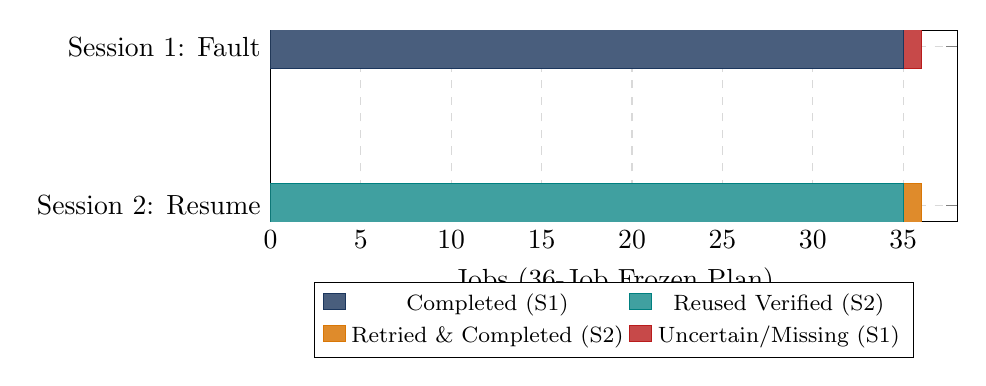
\begin{tikzpicture}
\begin{axis}[
  xbar stacked,
  bar width=16pt,
  width=0.85\textwidth,
  height=4.0cm,
  xlabel={Jobs (36-Job Frozen Plan)},
  symbolic y coords={Session 2: Resume, Session 1: Fault},
  ytick=data,
  xmin=0,
  xmax=38,
  legend style={at={(0.5,-0.32)}, anchor=north, legend columns=2, font=\footnotesize},
  grid=major,
  grid style={dashed, gray!30}
]
  \addplot[fill=navy!80, draw=navy] coordinates {(35,Session 1: Fault) (0,Session 2: Resume)};
  \addplot[fill=teal!75, draw=teal] coordinates {(0,Session 1: Fault) (35,Session 2: Resume)};
  \addplot[fill=amber!85, draw=amber] coordinates {(0,Session 1: Fault) (1,Session 2: Resume)};
  \addplot[fill=crimson!80, draw=crimson] coordinates {(1,Session 1: Fault) (0,Session 2: Resume)};
  \legend{Completed (S1), Reused Verified (S2), Retried \& Completed (S2), Uncertain/Missing (S1)}
\end{axis}
\end{tikzpicture}
\caption{Recorded recovery: Session~1 completes $35/36$ jobs and marks one \texttt{gpu-2} EOF as uncertain; Session~2 reuses $35$ verified results and completes \texttt{blue-9705} ($36/36$).}
\label{fig:fault}
\end{figure}

\subsection{Linux eBPF Kernel Telemetry}
An independent privileged recheck of \texttt{ops.ebpf\_tcp --port 22 --seconds 3} reported successful collector execution and zero retransmission events on host TCP sockets matching port~22, with $3.53\,\text{s}$ collector elapsed time. The raw record is \path{network-report/ebpf-live-recheck.json} under \path{docs/08-operations/}. It records neither dropped events nor the exact attachment window; it does not attribute events to an individual process, job, or VPN peer. The earlier reported $3.46\,\text{s}$ run has no retained raw capture. A zero host TCP event count does not establish zero Tailscale UDP packet loss.

\section{Limitations and Future Work}
\begin{itemize}
\sloppy
  \item \textbf{Scope:} Echo measurements cover coordinator-to-peer SSH paths, not all pairwise links. They are not evidence of full-mesh performance.
  \item \textbf{Sample Size \& Controls:} Each policy configuration represents one run, without live \texttt{network\_probe} files attached to the adaptive scorer; repeated interleaved runs are needed for statistical inference. Its history uses request times that already include network work; adding an RTT estimate when enabled can count some network time twice.
  \item \textbf{Transport Scope:} Tailscale encapsulates traffic over UDP, so host-level TCP retransmission hooks on SSH/loopback ports do not directly measure Tailscale UDP packet loss.
\end{itemize}

\end{document}
